\section{Методика~использования разработанного приложения}
\label{sec:usage}
Программное средство лексической и функциональной обфускации проектных описаний цифровых устройств представляет собой консольное приложение, которое может работать под управлением операционных систем семейства Windows и *nix. Корректная работа приложения гарантируется в ОС, перечисленных в разделе, описывающем анализ предметной области и укрупненную спецификацию требований. Данная методика использования программного сердства составлена с использованием операционной системы Arch Linux и симулятора терминала Sakura. Поскольку приложение является консольным и не содержит промежуточных состояний, в качестве управления используются аргументы, передаваемые при запуске приложения. Запуск приложения без аргументов(или с использованием аргументов -h или -help) и результат его работы представлены на рисунке \ref{fig:sec:usage:without_args}.

При запуске приложения в аналитическом режиме проверяется правильность кода, однако не выполняется его обфускация. Анализатор проверяет каждую сущность в дизайне и если она верна, то выводится соответствующее сообщение:

\begin{figure}[hbtp]
\centering
  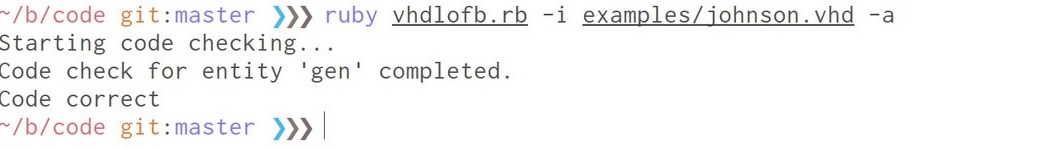
\includegraphics[scale=0.65]{analyze_success.jpg}
  \caption{ Запуск приложения в аналитическом режиме с корректным входным файлом }
  \label{fig:sec:usage:analyze_success}
\end{figure}

\afterpage{
  \begin{landscape}
  \thispagestyle{lscape}
  \begin{figure}[htbp]
  \centering
    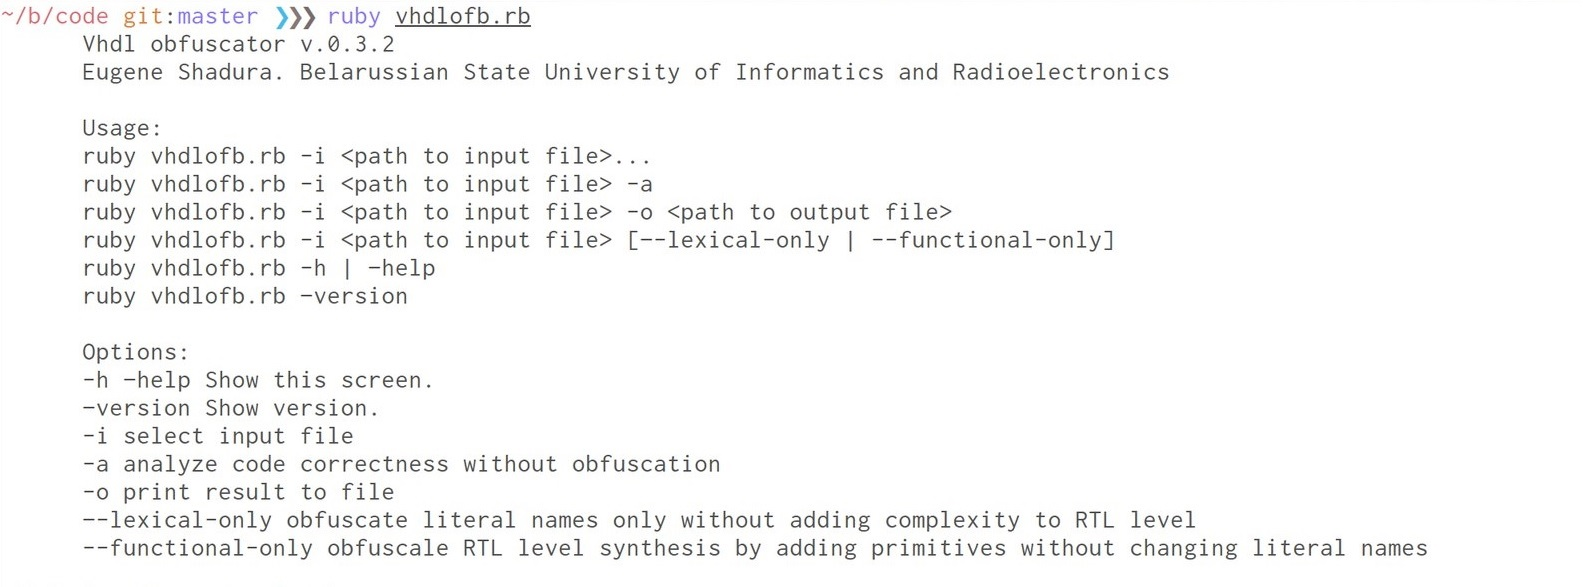
\includegraphics[scale=0.65]{without_args.jpg}
    \caption{ Запуск приложения без аргументов }
    \label{fig:sec:usage:without_args}
  \end{figure}
  \end{landscape}

}

Если же исходный код содержит какие-либо ошибки, то пользователь увидит сообщение с ошибкой, которое содержит символ, который привёл к ней:


\begin{figure}[ht]
\centering
  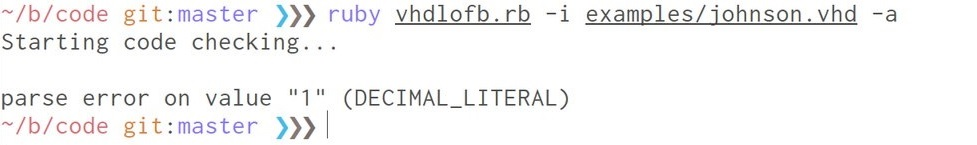
\includegraphics[scale=0.65]{analyze_error.jpg}
  \caption{ Запуск приложения в аналитическом режиме с некорректным входным файлом }
  \label{fig:sec:usage:analyze_error}
\end{figure}

\begin{landscape}
\thispagestyle{lscape}
\begin{figure}[ht]
\centering
  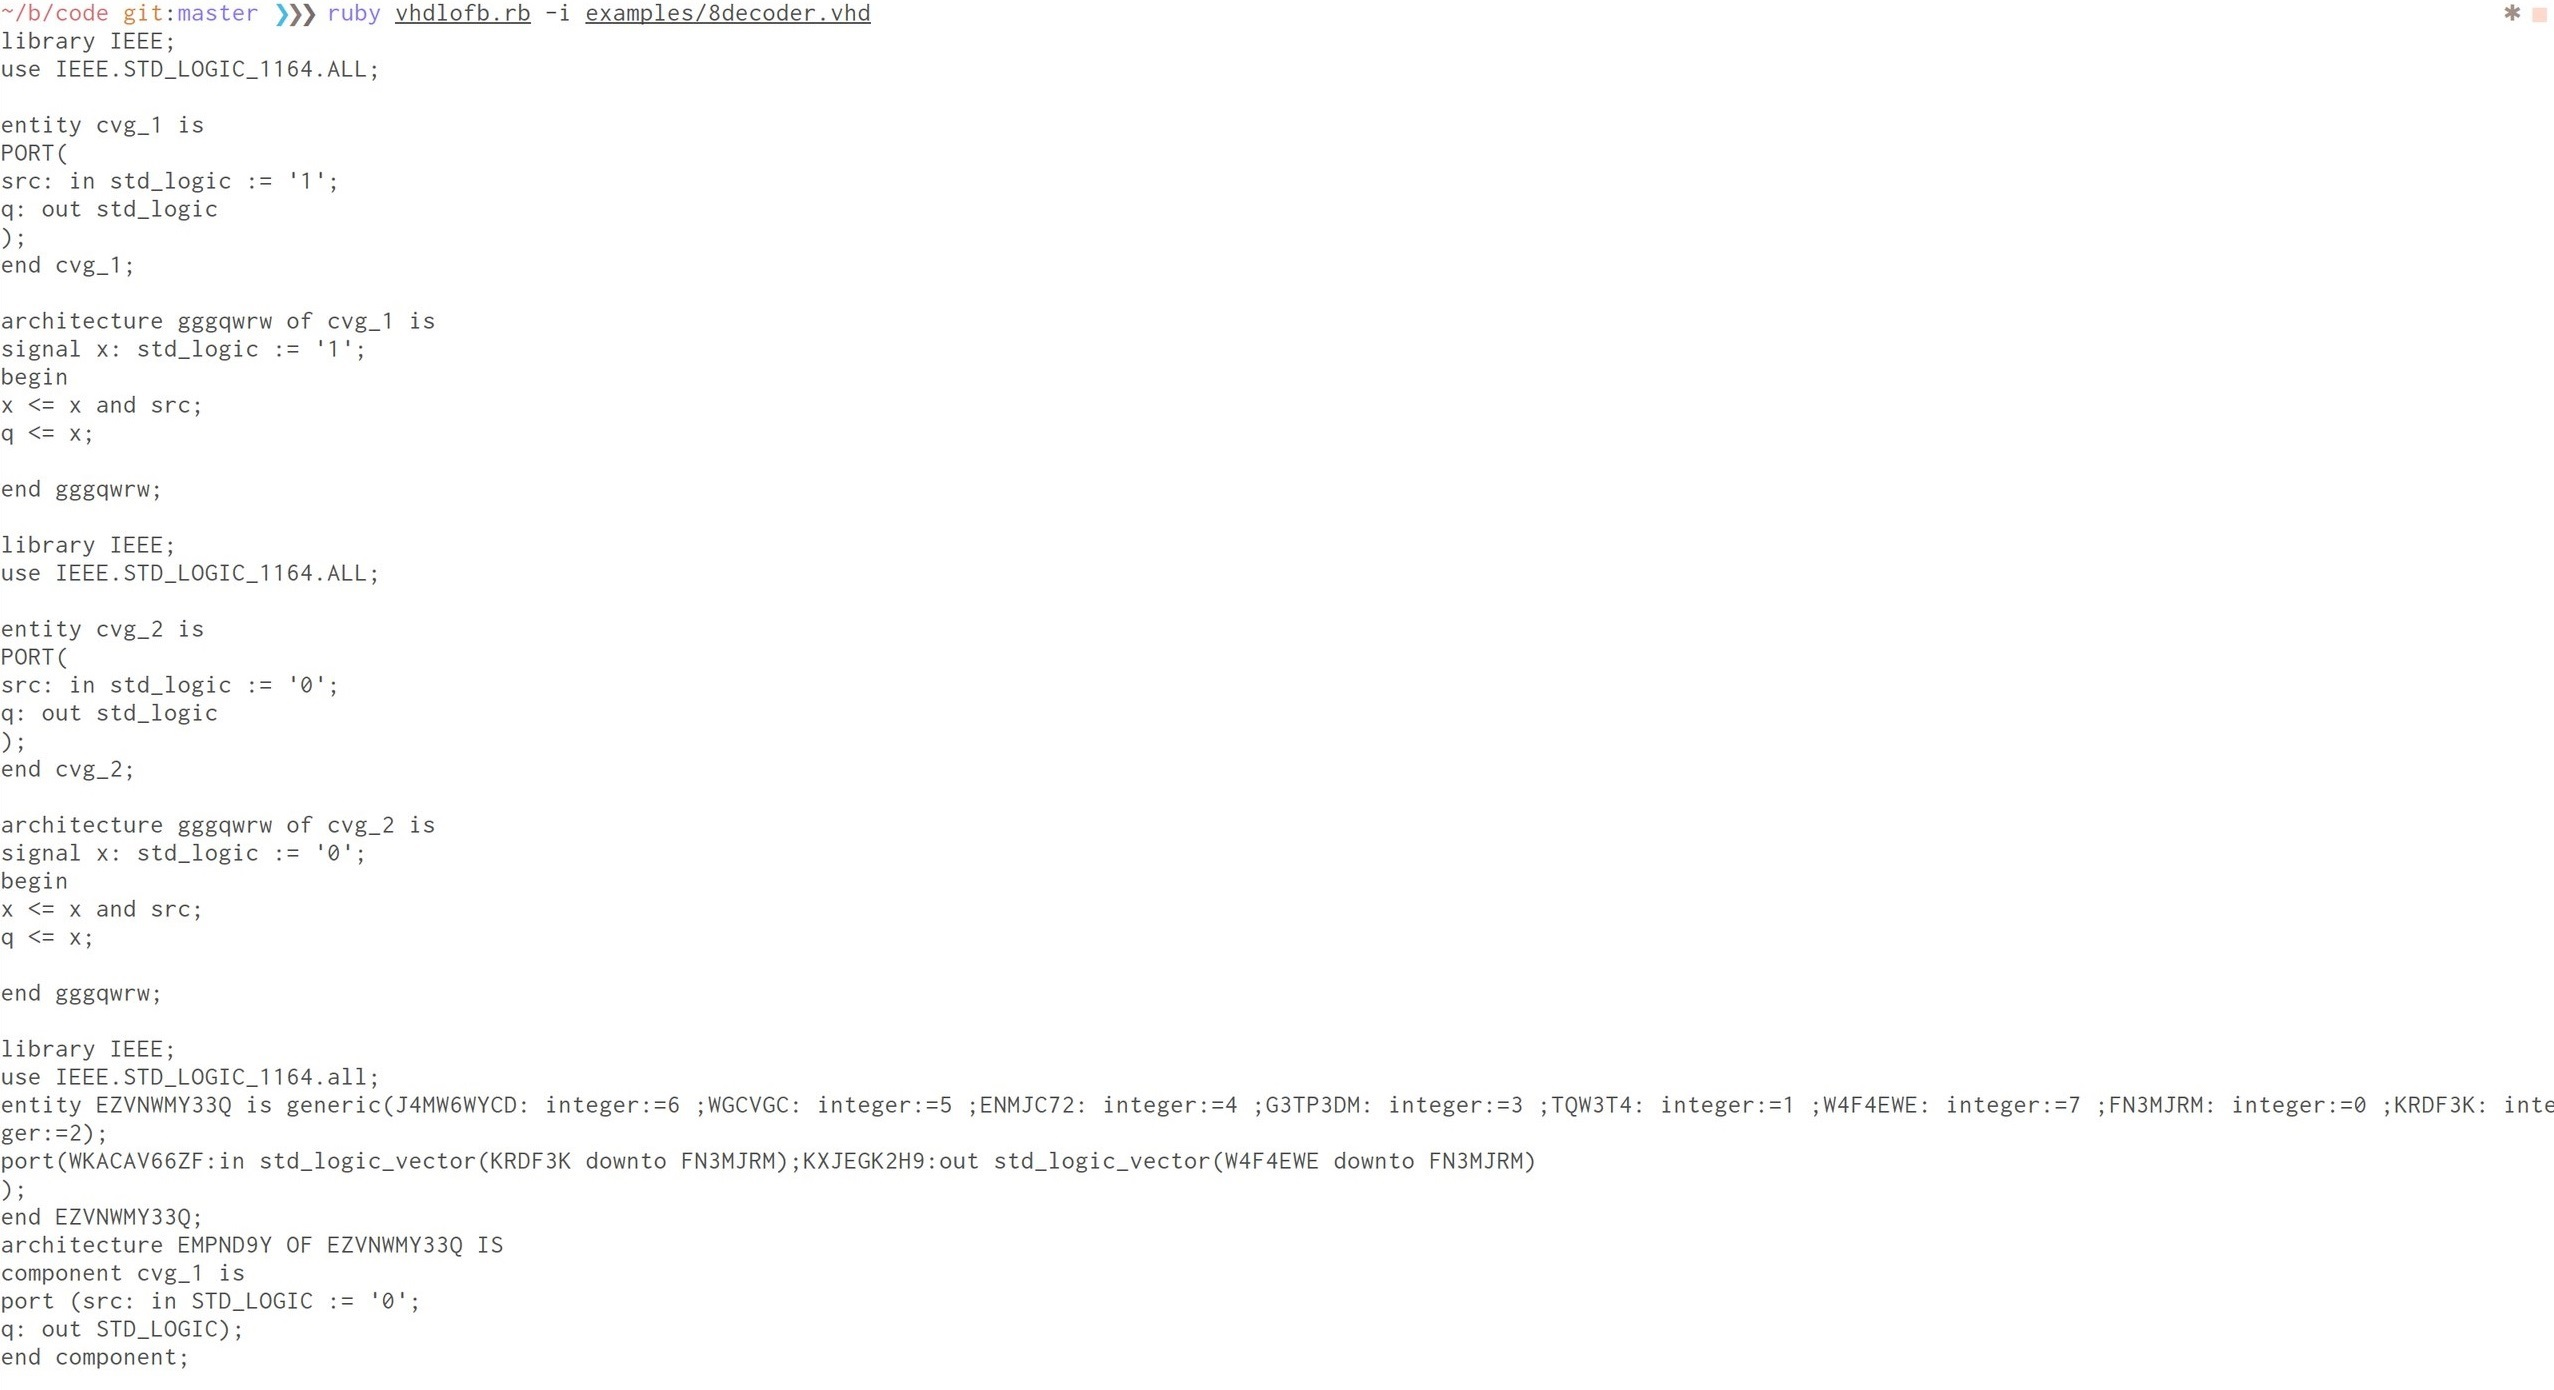
\includegraphics[scale=0.25]{without_output.jpg}
  \caption{ Запуск приложения без указания выходного файла }
  \label{fig:sec:usage:without_output}
\end{figure}
\end{landscape}

\clearpage

